\documentclass{article}

\usepackage{header}
\newcommand{\equivclass}[1]{%
  #1/{\sim}%
}

\usepackage[left=2cm,right=2cm, top=2cm,bottom=2cm,bindingoffset=0cm]{geometry}

\usepackage{hyperref}
\hypersetup{
    colorlinks=true,
    linkcolor=blue,
    filecolor=magenta,      
    urlcolor=cyan,
    pdftitle={Overleaf Example},
    pdfpagemode=FullScreen,
    }

\usepackage{graphicx}
\graphicspath{.}
\usepackage{algorithm}
\usepackage{algpseudocode}
% \usepackage{algpseudocodex}
% \usepackage[algo2e]{algorithm2e}
% \usepackage{algorithms}

\usepackage{hyperref}  % so the reference URLs and citations are clickable
\usepackage{csquotes}  % needed for biblatex for babel
\usepackage[backend=biber]{biblatex}
\addbibresource{bibliography.bib}

\usepackage{titlepage}

\setUDK{004.9}
\setToResearch

\setTitle{Приближение магнитудной функции метрического графа}

% Выбрать одно из трех:
% КТ1 -- \setStageOne
% КТ2 -- 
\setStageFinal
% Финальная версия -- 
% \setStageFinal
% \setStageOne
%\setStageTwo
%\setStageFinal

\setGroup{204}
%сюда можно воткнуть картинку подписи
% \setStudentSgn{\smash{\includegraphics[scale=0.25]{my-sig.png}}}
% \setStudentSgn{\includegraphics[scale=0.10]{my-sig.jpg}}
% \setStudentSgn{\smash{kjdfl}}
\setStudent{М.М.Марченко}
\setStudentDate{18.05.2023}
\setAdvisor{Всеволод Леонидович Чернышев}
\setAdvisorTitle{Доцент} %(научно-учебная лаборатория методов анализа больших данных)}
\setAdvisorAffiliation{НИУ ВШЭ, ФКН, Департамент больших данных и информационного поиска}
\setAdvisorDate{}
% \setGrade{}
%сюда можно воткнуть картинку подписи
\setAdvisorSgn{}
\setYear{2023}

\begin{document}

% Эта команда создает титульную страницу
\makeTitlePage

% Здесь будет автоматически генерироваться содержание документа
\tableofcontents

% Данное окружение оформляет аннотацию: краткое описание текста выделенным абзацем после заголовка
%\begin{abstract}
%    Проект в реализации теории,
%\end{abstract}

\section{Introduction}


\ \ \ \ Metric graph is a topological space which, simply put, represents a glued set 
of closed
intervals. Unlike combinatorial weighted graph it is not discrete, but 
continuous, containing not only
vertices, but also all points on the edges. \\

For a given metric graph we can calculate a magnitude function, object 
originally coming from category theory. Being a generalized notion of size,
magnitude function is defined for enriched categories, and metric graph is a type of metric space, which, in turn, is a type of enriched category. \\

\textbf{Magnitude function of two points space:}
\begin{center}
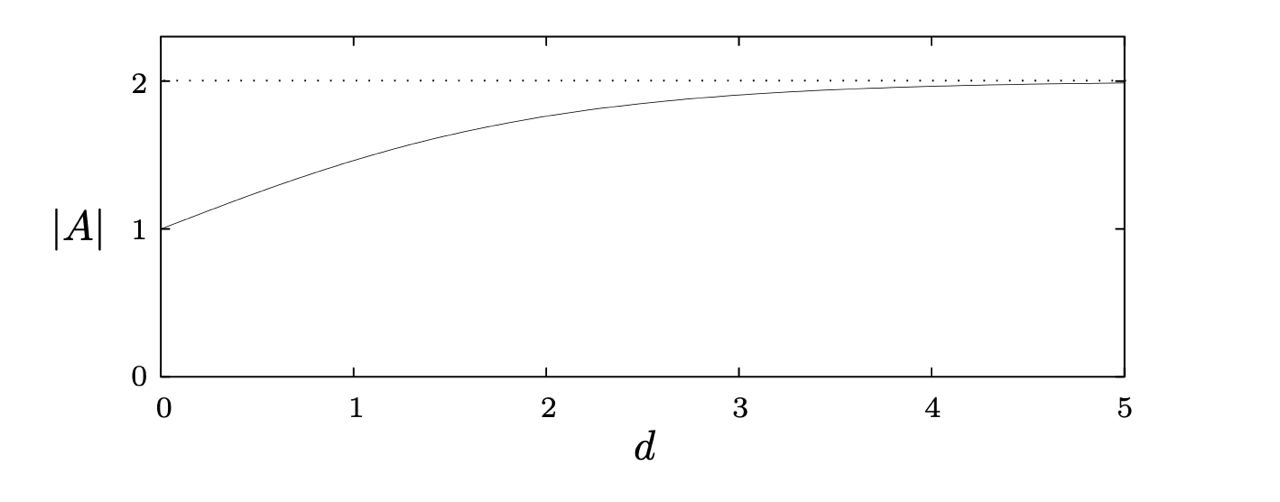
\includegraphics[width=.4\textwidth]{2dots}
\end{center}

\ \ \ \ As calculated by \textcite{Leinster_2012} the magnitude function of an interval of length $l$ equals $\frac{lt}{2} + 1$,
while magnitude of two points space with distance $l$ between them equals $\frac{2}{1 + e^{-lt}}$.
Calculation of magnitude function of the first object has some non-trivial mathematical steps,
while calculation of the magnitude function of the second object is a simple algorithmic task of finding a reverse 4 element matrix.  
Moreover the resulting values of the magnitude function don't seem to have some sort of simple relation and magnitude of interval can not be simply calculated from magnitude of its endpoints.\\ 

But $l \rightarrow \frac{l}{2} + 1$ is a rather simple function which might have been guessed from the computer simulations. 
\\


Magnitude of a combinatorial graph was already studied by \textcite{LEINSTER_2017},
but as we see in the case of interval of length $l$ and two discrete points with 
distance $l$ between them, studying magnitude of the continuous space is a whole different problem.
\\

In this work we present the results of computer simulations for different metric
graphs and the conjecture about behavior of the magnitude function derived from them,
which goes along with all the experiments so far. 
\\

The work is structured in the following way: in the Background section we will 
give definitions of magnitude function and metric graph, explain their relation
and explain why magnitude of a metric graph is defined and how it can be calculated.
\\

Then in the Conjectures section we explain the following 2 suggestions:
\\

1. Magnitude function of a metric graph asymptotically satisfies the inclusion-exclusion principle. \\

2. Magnitude of a metric graph asymptotically is equal to $\frac{t \cdot length}{2} + \chi(\mathcal{G})$, where $\chi$ is Euler characteristic and $length$ is sum of edges lengths.
\\

In the Experiments and their interpretations we prove 2nd hypothesis for particular cases of metric graphs, 
explain how we approximate magnitude 
and then go through all the graphs we experimented on. For each of them we give the simulations 
result and then explain how it aligns with the conjectures (so we decompose the graphs to simpler 
parts to use the inclusion-exclusion principle) and also show how the result aligns with already 
known magnitudes and theorems. 
\\ 

After that in Methods we go through details about the way we calculated magnitude function 
numerically and then explain the unsuccessful way how we tried to approximate magnitude. 
\\

\section{Background}
\subsection{Definitions}
\subsubsection{Metric Graph}

\ \ \ \ As already mentioned in the introduction, we can intuitively understand metric graphs as 
weighted graphs which, besides vertices, also contain all the points on the edges. 
The other intuitive understanding would be a set of intervals joined by their ends,
thus forming a graph. \\

A stricter definition, originally coming from \textcite{MG1}, is given below. 

$$\mathcal{E} \coloneqq \bigsqcup \ [0, l_{e}] \mid e \in E, \  l_e \in (0, \infty) \text{, where } E \text{ is a countable set and } \bigsqcup \text{ is a disjoined topological union.}$$
$$\text{The notation for elements of $\mathcal{E}$ is: }(x, e) \in \mathcal{E} \iff e \in E \land x \in [0, l_e]$$
$$\mathcal{V} \coloneqq \bigsqcup \ \{(0, e), (l_e, e)\}$$
$$\text{On } \mathcal{V} \text{ we define an equivalency relation } \sim_{\mathcal{V}} \text{with classes of equivalency } \{V_i\} \text{ (each represents a vertex)}$$
$$\text{On } \mathcal{E} \text{ we define an equivalency relation } \sim_{\mathcal{E}} \ \mid (x_1, e_1) \ \sim_{\mathcal{E}} (x_2, e_2) \iff x_1 = x_2; e_1 = e_2 \text{ or } (x_1, e_1) \sim_{\mathcal{V}} (x_2, e_2)$$
\begin{definition}
    $\mathcal{G} = \mathcal{E} \ \slash \sim_{\mathcal{E}} \text{ is a \textbf{metric graph} with vertices } \mathcal{V} \ \slash \sim_{\mathcal{V}}$
\end{definition}
\subsubsection{Magnitude}

First we will give a definition of magnitude for a finite metric space, then two equivalent definitions for
compact positive definite metric spaces, taken from \textcite{Leinster_2012}. 
\begin{definition}
\item 
    $\text{Let $X$ be a finite metric space with metric $d$.}$
\item
    $$\text{Magnitude of $X$ is } \mathcal{M}(X) \coloneqq \sum_{x \in X} w_x \text{, where } w_x \in \mathbb{R} \text{ and } \forall x \in X : \sum_{x' \in X} w_x \cdot e^{-d(x, x')} = 1$$
\end{definition}
\begin{remark}
\item
    $\text{If $Z$ is a $|X| \cross |X|$ matrix, with values $Z_{i, j} = e^{-d(x_i, x_j)}$, where $x_i, x_j \in X$ and Z is invertible, then:}$
\item
    $$\mathcal{M}(X) = \sum_{i, j} (Z^{-1})_{i, j} $$
\end{remark}
\begin{definition}
\item 
    $\text{Let $X$ be a positive definite metric space, then:}$
    $$\mathcal{M}(X) = \sup\{\mathcal{M}(Y) : Y \subset X \text{ and $|Y| < \infty$}\}$$
\end{definition}
\begin{definition}
    (equivalent to definition 3)
\item 
    $\text{Let $X$ be a positive definite metric space and $\{X_i\} \text{ its subsets } : |X_i| < \infty \text{ and } X_i \rightarrow X$ in Hausdorff metric then:}$ 
    $$\mathcal{M}(X) = \lim_{i \rightarrow \infty} \mathcal{M}(X_i)$$
\end{definition}
\subsubsection{Magnitude function}
\begin{definition}
    $\text{If } X \text{ is a metric space with metric $d(x, y)$ and $t \in (0, \infty)$ then } tX \text{ is a metric space with metric } t \cdot d(x, y)$
\end{definition}
\begin{definition}
    $f_{\mathcal{M}} : (0, \infty) \rightarrow \mathbb{R} \text{ is a magnitude function of X, if }$
    $$f_{\mathcal{M}}(t) = \mathcal{M}(tX)$$
\end{definition}

\textbf{Illustration of magnitude function for a three point space with the following distances:}
\\ Note how the values of the magnitude function correspond to the number of points seen if we change the perspective: first we see 1 point, then 2 as we get closer but still see two of them as one, then 3.
\begin{center}
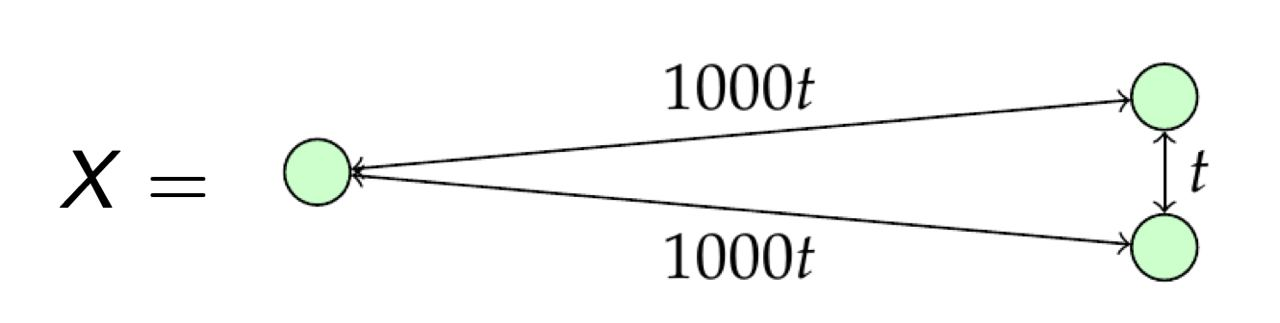
\includegraphics[width=.4\textwidth]{3dots} \\ 
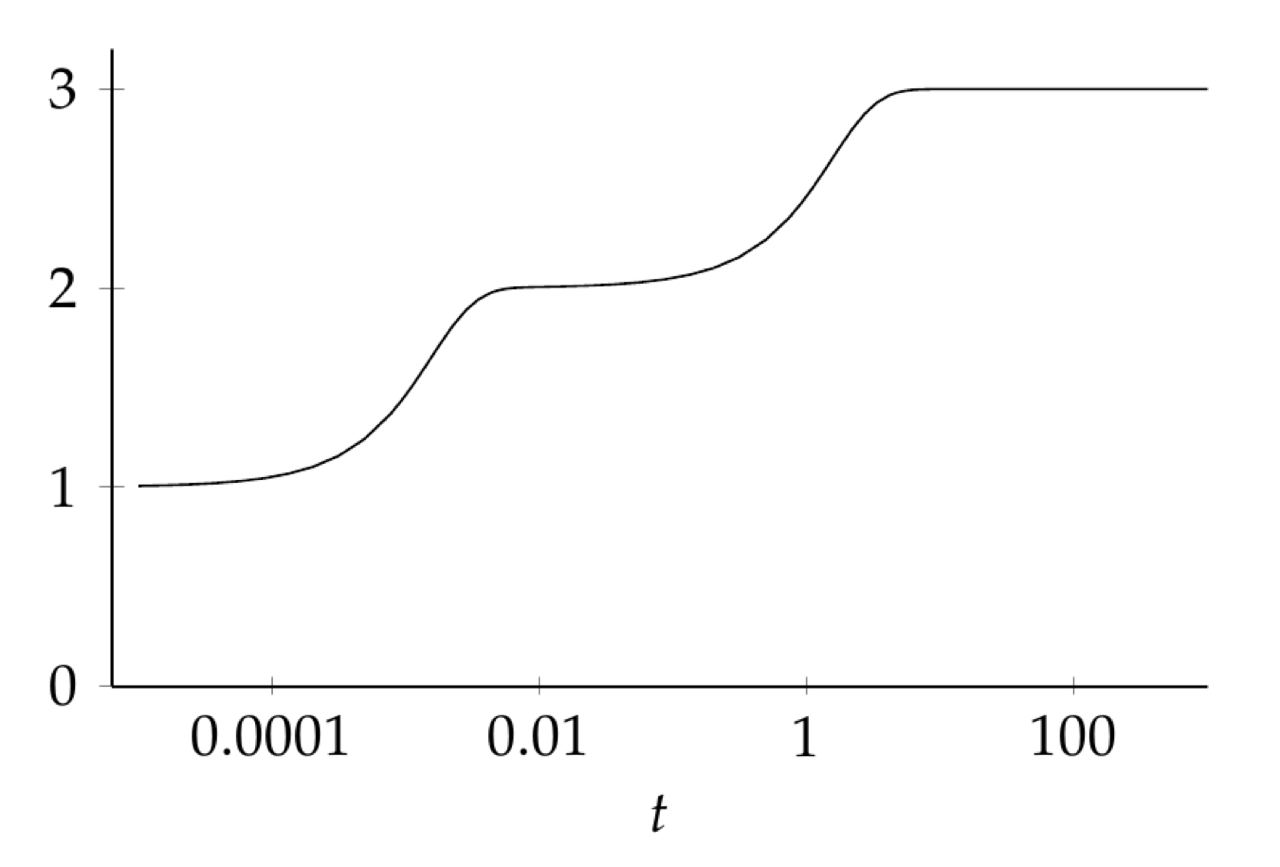
\includegraphics[width=.35\textwidth]{mfunc3dots}
\end{center}
\subsection{Metric graph as a compact metric space}

Metric graphs are metric spaces with metric equivalent to shortest path between two points.
Let's quickly define it as it appears in \textcite{MG1}.

$$
    d_{\mathcal{E}}((x_1, e_1), (x_2, e_2)) =
    \begin{cases}
        |x_1 - x_2|, & \text{ if } e_1 = e_2 \\
        \infty, & \text{otherwise }
    \end{cases}
$$
$$ 
  d_{\mathcal{G}}(\xi, \theta) = \inf \{\sum_{i = 1}^{k} d_{\mathcal{E}}(\xi_i, \theta_i)\} \quad \xi_i, \theta_i \in \mathcal{E}
$$

In our case we consider graphs with $|E| < \infty$, thus we can easily prove that it's a metric space and moreover a compact metric space. 
\\ \\ \textbf{Metric graph is a metric space}
    \\
    $$
    1. \ d_{\mathcal{G}}(x, y) = 0 \iff x = y$$ 
    $$
    2. \ d_{\mathcal{G}}(x, y) = d_{\mathcal{G}}(y, x)
    $$
    $$\text{1-2 are obvious from the definition of } d_{\mathcal{E}}, d_{\mathcal{G}} \text{ as either distances (which is interval metric)}$$
    $$\text{between points on the interval, either their sum.}$$
    $$
    3. \ d_{\mathcal{G}}(x, y) \leq d_{\mathcal{G}}(x, z) + d_{\mathcal{G}}(z, y)
    $$
    $$
    \text{3 is also obvious since } x \rightarrow z \rightarrow y \text{ is also a valid path, thus can't be less than infimum.}
    $$
\\ \\ \textbf{Metric graph is a compact metric space}

$$
\text{Since } |E| < \infty \text{ for any sequence of points we can find an edge which contains infinite subsequence and since edge is}$$
$$\text{an interval which is a compact, it has a convergent subsequence, thus metric graph is a compact.}
$$

\section{Conjectures}

The pattern that we observed in the behavior of the magnitude function during 
computer simulations is formulated below:

\begin{hypothesis}
    The magnitude of the metric graph asymptotically satisfies the inclusion-exclusion principle.
\end{hypothesis}
Similar conjecture about subsets of Euclidean space was made in \textcite{Leinster_2012}.
But since metric graphs are not always subsets of Euclidean space and to our knowledge
this conjecture has not been proven, our result is a contribution.
\\

More strictly the hypothesis states:
$$\forall A, B . \exists q_A, q_A : \mathcal{M}_A(t) = P_A(t) + q_A(t), \mathcal{M}_B(t) = P_B(t) 
+ q_B(t) \text{, where } q_A(t) \rightarrow 0, q_B(t) \rightarrow 0$$


If the conjecture is right we can derive magnitude of any graph by decomposing 
it step by step to simpler elements: as shown in section Overview of the relevant results,
we already know magnitude of finite number of points, magnitude of an interval,
magnitude of a cycle and magnitude of a tree.

Moreover, stronger conjecture would be the following one:

\begin{hypothesis} If $\mathcal{G}$ is a metric graph with edges $\mathcal{E}$, then
    $\mathcal{M}_{\mathcal{G}} = \frac{l \cdot t}{2} + const$, where 
    $l = \sum_{e \in \mathcal{E}} length_e$ and $const =$ Euler characteristic of $\mathcal{G}$. 
\end{hypothesis}

This conjecture is also consistent with all the simulation results.
Besides, since Euler characteristic $\chi = |\mathcal{V}| - |\mathcal{E}|$ \textcite{_awniczak_2020}
satisfies the inclusion-exclusion principle with some restrictions, 
and both cycle magnitude and edge magnitude satisfy 2nd theorem, it might be corollary of the 1st theorem.
\\

\textbf{We did not obtain any proofs concerning the 1st hypothesis. 
2nd hypothesis proofs for spectial cases of the metric graphs can be found in section 4.3. }

\section{Experiments and their interpretations}
\subsection{Approximation of the magnitude function}

Here we will briefly explain how the magnitude function was approximated.
Pseudocode, relevant computation details and all links can be found in the Methods section. 
Code can be found on \href{https://github.com/mmanchkin/magnitude}{Github} and in
\href{https://colab.research.google.com/drive/17Wlg996wKO1tZD9EBfn9G5qiL2nD_5LM?usp=sharing}{Colab}.
\\

For a fixed $t$ and a fixed graph $\mathcal{G}$ we approximate a continuous metric graph with it's discrete subsets
--- finite combinatorial graphs, which we get by dividing each edge into equal parts.
\\

For each graph in this sequence $\{\mathcal{G}_{k}\}$ we calculate magnitude ($\mathcal{M}_k(t)$) as in
remark 1: as sum of elements of $Z^{-1}$, where $Z_{i, j} = e^{-t \cdot d_{\mathcal{G}_k}(v_i, v_j)} \mid v_i, v_j \in \mathcal{V}_k$. \\

As follows from the 4th definition:
$$ \mathcal{M}(t) = \lim_{k \to \infty} \mathcal{M}_k(t)$$

Range of $k$ and $t$ is specified and explained in the Methods section.
\\

We run this algorithm on several $t = {t_1, t_2, ...}$ and draw a plot with the measured
magnitude: \\ $\mathcal{M}_{k} = (t_1, \mathcal{M}_k(t_1)), (t_2, \mathcal{M}_k(t_2)), ...$. 

After that we guess the real magnitude function: $\mathcal{M}_{guessed}(t)$, and compare the
experiment result and our guess using two plots, described below.
\\

The first one draws $\mathcal{M}_{guessed}(t)$ and $\mathcal{M}_{k}$. The $length$ of the graph equals to the sum of
 its weighted edges. 
\\

The second plot represents the convergence delta --- by which we mean 
$|\mathcal{M}_k(t) - \mathcal{M}_{k - 1}(t)|$, compared to the difference between
the experiment result and the guessed magnitude function:  ($|\mathcal{M}_{guessed}(t) - \mathcal{M}_k(t)|$),
where $\mathcal{M}_k(t)$ is the magnitude measured for the last finite graph in
the sequence (the one with the biggest number of vertices).

As t gets bigger, the pairwise distances between the points of the combinatorial
graph grow too. This leads to the superlinear growth of the numerical error, because
the magnitude is calculated by inverting a matrix with elements equal to the exponent
to the power of negated pairwise distances. That's why we need some reference
to check that they grow proportionally.
In our case as a reference we use convergence delta since it perfectly shows how close
the magnitude is to the real value (similar to the Cauchy convergence).
\\

Note that all the magnitudes we studied ended up in the $\frac{t \cdot length}{2} + const$
neighbourhood, so in the most of the cases the second plot was more useful. The
next example shows the difference between the plot when the $const$ was guessed
correctly compared to the plot with an incorrect $const$.

\begin{center}
    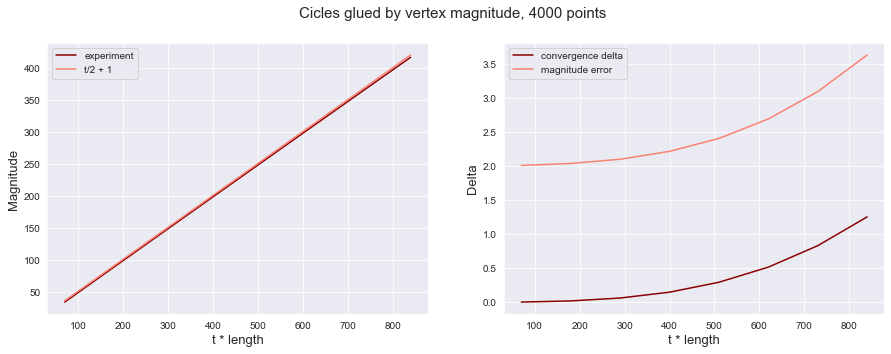
\includegraphics[width=\textwidth]{cicles_glued_by_vertex_wrong} Example 
    where the $const$ was guessed wrong: the plot is still similar to $\frac{t}{2}$
    but in comparison to convergence delta we can see, that the $const$ should be decreased by 2. \
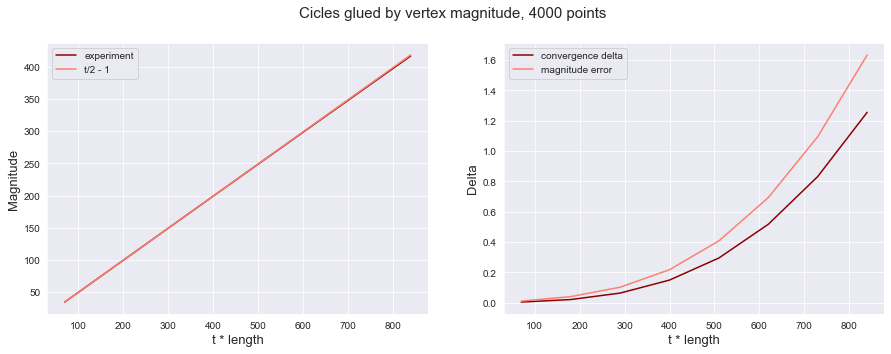
\includegraphics[width=\textwidth]{cicles_glued_by_vertex_right} This example illustrates
    the right guess - note how convergence delta correlates with difference between real
    magnitude and experiment results.
\end{center}


\subsection{Overview of the relevant results}

To interpret the experiments results we will briefly overview the relevant
results.

First of all, the magnitude of the most basic objects: let $p_1$ be 1 point, $p_1\leftrightarrow p_2$ --- 2 points on distance equal to $l$. Then:

$$\mathcal{M}_{p_1}(t) = 1$$
$$\mathcal{M}_{p_1\leftrightarrow p_2}(t) = \frac{2}{1 + e^{-t \cdot l}}$$

These magnitudes, as well as magnitude of any finite metric space, are easily computed
without any analytic steps by inverting one matrix and summing the elements
of the result.
\\

For the subsets of the Euclidean space known results
are the magnitude of an interval of length $l$ and a circle of circumference $l$ (\textcite{Leinster_2012}):

$$\mathcal{M}_{\text{interval of length $l$}}(t) = \frac{l \cdot t}{2} + 1$$
$$\mathcal{M}_{\text{circle of circumference $l$}}(t) = \frac{l \cdot t}{2} + q(t) \text{, where } \lim_{t \rightarrow \infty} q(t) = 0$$

Another interesting result, \textcite{Leinster_2012}:

\begin{theorem}
    If X is a finite metric space with n points then $\lim_{t \rightarrow \infty} \mathcal{M}_X(t) = n$.
\end{theorem}
 

Note that in the case of a circle the metric does not need to be euclidean --- magnitude is the same
for the arc length metric, which would be useful to us in the case of a cycle.


Both of these calculations require non-trivial steps (and asymptotic analysis in the case of circle)
but as we can see the dependence is simpler than in the case of two points and could have been guessed from simulations,
see sections Intervals and Cycles.
\\

As already mentioned in the third section, in \textcite{Leinster_2012} there is
a similar conjecture to the one stated in this paper: "the magnitude of subsets of
Euclidean space asymptotically satisfies the inclusion-exclusion principle". \\

The other important result and its two corollaries are taken from \textcite{LEINSTER_2017}.

\begin{theorem}
Let $X$ be a graph, with subgraphs $G$ and $H$ such that $G \cup H = X$. Suppose
    that $G \cap H$ is \textit{convex} in $X$ and that $H$ \textit{projects} to $G \cap H$. Then:
    $$\mathcal{M}_X = \mathcal{M}_G + \mathcal{M}_H - \mathcal{M}_{(G \cap H)}$$
\end{theorem}
\begin{corollary}
    Let $G$ and $H$ be graphs and $G \vee H$ is the graph obtained by gluing them
    together with one point. Then:
    $$\mathcal{M}_{G \vee H} = \mathcal{M}_{G} + \mathcal{M}_{H} - 1$$
\end{corollary}

\begin{corollary}
    Let $X$ be a tree, with subtrees $G$ and $H$ such that $G \cup H = X$. Then:
    $$ \mathcal{M}_X = \mathcal{M}_G + \mathcal{M}_H - \mathcal{M}_{G \cap H}$$
\end{corollary}

\subsection{Hypothesis proofs for particular cases}

\subsubsection{Cycle and interval}

Cycle and interval satisfy the 2nd hypothesis:

$$\chi_{cycle} = 0; \  \chi_{interval} = 1$$ From \textcite{Leinster_2012} (circle with an arc distance metric):
$$\mathcal{M}_{circle} = \mathcal{M}_{cycle} = \frac{l \cdot t}{2} + q = \frac{l \cdot t}{2} + \chi_{cycle} + q \text{, where} \lim_{t \rightarrow \infty} q = 0$$
$$\mathcal{M}_{interval} = \frac{l \cdot t}{2} + 1 = \frac{l \cdot t}{2} + \chi_{interval}$$

\subsubsection{Metric graphs glued by vertex}

\begin{theorem}
    Let $X, G, H$ be metric graphs such that $X = G \vee H$ (glued by vertex $v_1$)
    and $\mathcal{M}_G, \mathcal{M}_H$ satisfy the 2nd hypothesis. Then $\mathcal{M}_{X}$
    also satisfy the 2nd hypothesis.
\end{theorem}

\textbf{Proof:} \\

1. $X \text{ is a metric graph } \Rightarrow$
$$\Rightarrow \chi_X = |V_X| - |E_X| = |V_G \cup V_H| - |E_G \cup E_H| = |V_G| + |V_H| - 
|V_G \cap V_H| - |E_G| - |E_H| = \chi_G + \chi_H - 1$$

2. 
Let $\{G_i\}, \ \{H_i\}$ be sequences of combinatorial subgraphs of $G$ and $H$ accordingly, such that:
$$v_1 \in G_i, H_i; \ \lim_{i \rightarrow \infty} G_i = G; \  \lim_{i \rightarrow \infty} H_i = H$$
Then:
$$\lim_{i \rightarrow \infty} G_i \cup H_i = X \ \Rightarrow \ \mathcal{M}_X =
\text{ [by 4th definition] } = \lim_{i \rightarrow \infty} \mathcal{M}_{G_i \cup H_i} = $$ 
$$ = \text{ [by 2nd theorem since vertex is convex and projection of any graph] } = $$
$$ = \lim_{i \rightarrow \infty} (\mathcal{M}_{G_i} + \mathcal{M}_{H_i} - 
\mathcal{M}_{G_i \cap H_i}) = \lim_{i \rightarrow \infty} \mathcal{M}_{H_i} +
\lim_{i \rightarrow \infty} \mathcal{M}_{E_i} - 1 = \text{ [by assumption] } = $$
$$ = \frac{l_G \cdot t}{2} + \chi_G + q_G + \frac{l_H \cdot t}{2} + \chi_H + q_H - 1 = 
\frac{l_X \cdot t}{2} + (\chi_G + \chi_H - 1) + (q_G + q_H) = $$ 
$$ = \frac{l_X \cdot t}{2} + \chi_X + q \text{, where } q \rightarrow \infty$$

\subsubsection{Graphs with $\leq 1$ cycle}

All of the following corollaries immedeately follow from the 3rd theorem,
since we can step by step construct these metric graphs from either a cycle or
an edge by gluing new edges or cycles to the vertices of the existing graph. 

\begin{corollary}
    Any \textbf{metric tree} satisfy the 2nd hypothesis.
\end{corollary}

\begin{corollary}
    Any \textbf{metric graph with 1 cycle} satisfy the 2nd hypothesis.
\end{corollary}

\begin{corollary}
    Any metric graph where all cycles intersect in 1 point, satisfy the 2nd hypothesis.
\end{corollary}


\subsection{One edge}

\begin{center}
    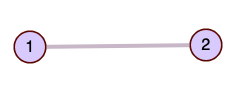
\includegraphics[width=0.2\textwidth]{interval_exp}
\end{center}

\textbf{Asymptotic magnitude from simulations:}
$$\mathcal{M}_{edge} = \frac{l \cdot t}{2} + 1$$

\textbf{Simulations plot:}

\begin{center}
    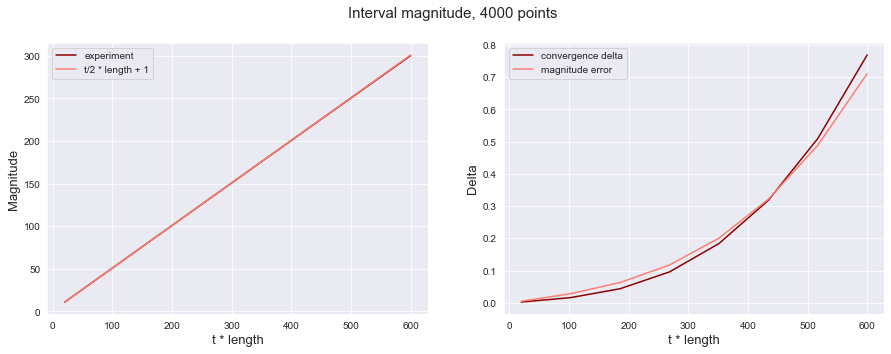
\includegraphics[width=\textwidth]{interval_plot}
\end{center}


\textbf{Hypothesis testing:}  consistent, see the 4.3.1 section. 

\subsection{Trees}

\begin{center}
    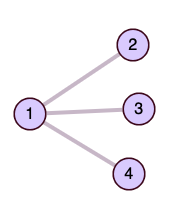
\includegraphics[width=0.15\textwidth]{bundle1_exp} \ \ \ \ \ \  
    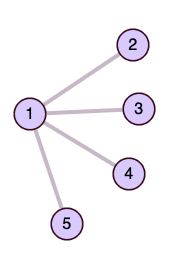
\includegraphics[width=0.15\textwidth]{bundle2_exp} \\
    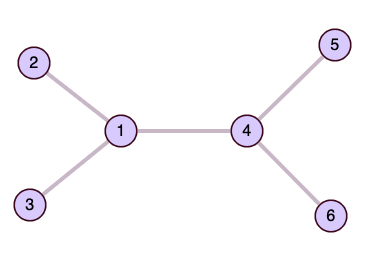
\includegraphics[width=0.3\textwidth]{comb_bundle1} \ \ \ \ \ \ 
    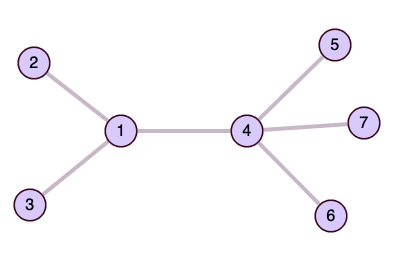
\includegraphics[width=0.3\textwidth]{comb_bundle2}
\end{center}

\textbf{Asymptotic magnitude from simulations (for all of the configurations):}
$$\mathcal{M}_{tree} = \frac{l \cdot t}{2} + 1$$

\textbf{Simulations plot:}

(For one of the configurations, other plots can be found in colab)

\begin{center}
    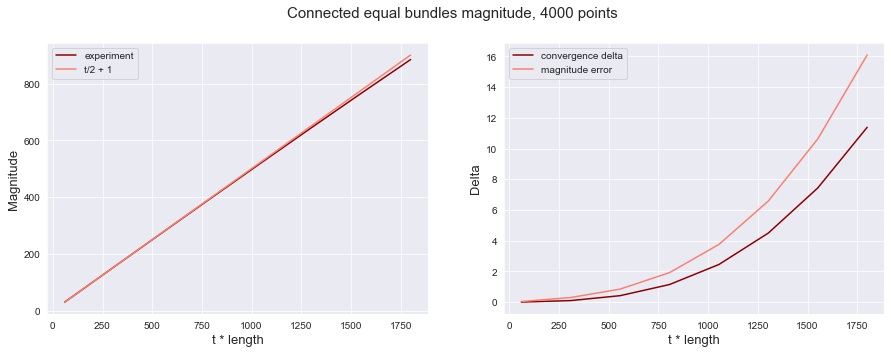
\includegraphics[width=\textwidth]{comb_bundle_plot}
\end{center}

\textbf{Hypothesis testing:} consistent, see the 4.3.3 section. 

\subsection{Cycle}
\begin{center}
    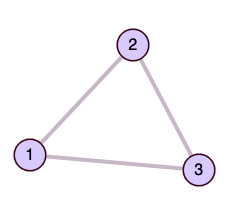
\includegraphics[width=0.2\textwidth]{cicle_exp}
\end{center}


\textbf{Asymptotic magnitude from simulations:}

$$\mathcal{M}_{cycle} = \mathcal{M}_{circle} = \frac{l \cdot t}{2}$$

\textbf{Simulations plot:}

\begin{center}
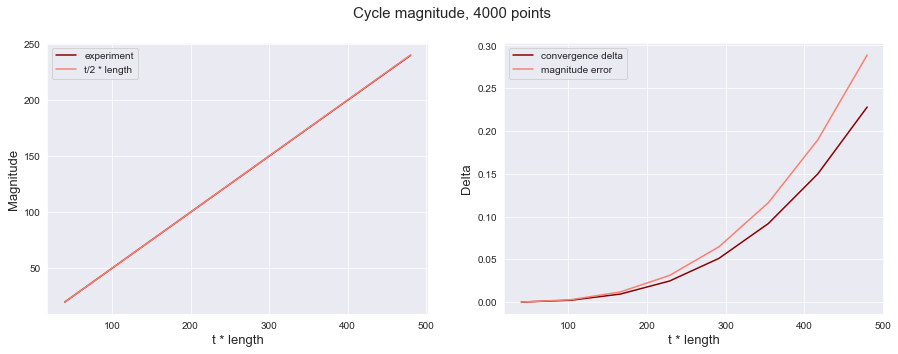
\includegraphics[width=\textwidth]{cycle_plot} 
\end{center}

\textbf{Hypothesis testing:} consistent, see the 4.3.1 section. 

\subsection{Cycles combined with trees}
\begin{center}
    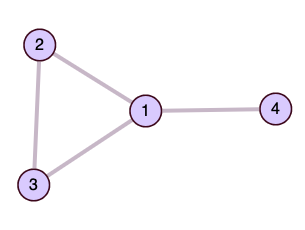
\includegraphics[width=0.2\textwidth]{cicle_tree1_exp}
    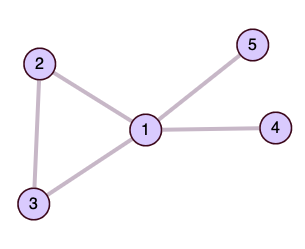
\includegraphics[width=0.2\textwidth]{cicle_tree2_exp}
\end{center}

\textbf{Asymptotic magnitude from simulations:}
\\

$$\mathcal{M}_{cycle \ + \ tree} = \frac{l \cdot t}{2}$$



\textbf{Hypothesis testing:} consistent, see the 4.3.3 section. 


\subsection{Combinations of 2 cycles}
\subsubsection{Glued by vertex}

\begin{center}
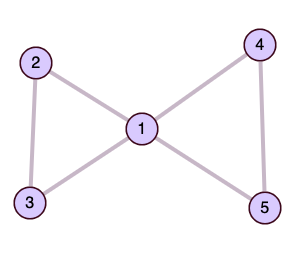
\includegraphics[width=0.3\textwidth]{2cicles_v_exp} 
\end{center}

\textbf{Asymptotic magnitude from simulations:}
\\

$$\mathcal{M}_{2cycles-1vertex} = \frac{l \cdot t}{2} - 1$$


\textbf{Consistent with the 1st hypothesis:} when we glue 2 cycles with 1 vertex by inclusion-exclusion
principle: $$\mathcal{M}_{new \ graph} = \mathcal{M}_{cycle1} + \mathcal{M}_{cycle2} -
\mathcal{M}_{connecting \ point} = \frac{l_1 \cdot t}{2} + \frac{l_2 \cdot t}{2} - 1= \frac{l \cdot t}{2} - 1$$ 
\\

\textbf{Consistent with the 2nd hypothesis:} see the 4.3.3 section. 

\subsubsection{Glued by edge}
\begin{center}
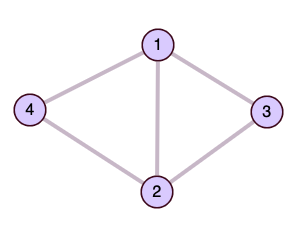
\includegraphics[width=0.3\textwidth]{2cicles_e_exp}
\end{center}

\textbf{Asymptotic magnitude from simulations:}

$$\mathcal{M}_{2cycles-1edge} = \frac{l \cdot t}{2} - 1$$

\textbf{Simulations plot:}
\begin{center}
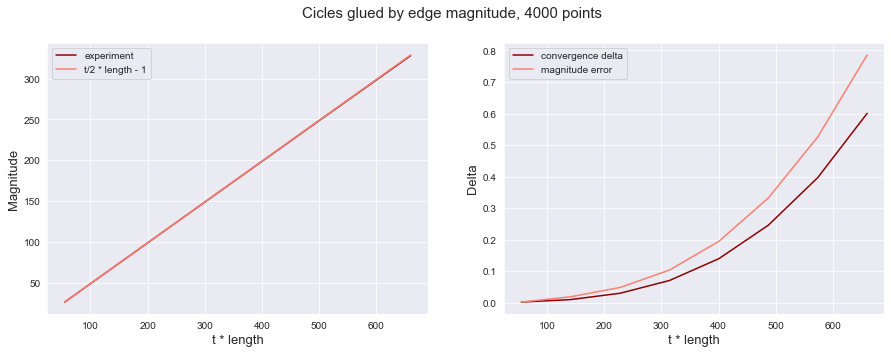
\includegraphics[width=\textwidth]{cicles_glued_by_edge}
\end{center}

\textbf{Consistent with the 1st hypothesis:} \\

1. When we glue 2 cycles by edge by inclusion-exclusion
principle: $$\mathcal{M}_{new \ graph} = \mathcal{M}_{cycle1} + \mathcal{M}_{cycle2}
- \mathcal{M}_{connecting \ edge} = \frac{l_1 \cdot t}{2} + \frac{l_2 \cdot t}{2} - 
(\frac{l_3 \cdot t}{2} + 1) = \frac{l \cdot t}{2} - 1$$
\\

2.
Another way to apply conjecture is to view this graph as a tree glued to a cycle
by two points (1-2-3 as a cycle, 1-4-2 as a tree, and 1,2 as their intersection). Then:

$\mathcal{M}_{new \ graph} = \mathcal{M}_{cycle} + \mathcal{M}_{tree}
- \mathcal{M}_{p_1 \leftrightarrow p_2} = \frac{l_1 \cdot t}{2} + \frac{l_2 \cdot t}{2} + 1 - 
\mathcal{M}_{p_1 \leftrightarrow p_2} = \frac{l \cdot t}{2} - 1 + q \text{, where } q \rightarrow 0$,
since from Theorem 3: $\mathcal{M}_{n \ points} \rightarrow n$ 
\\

Thus in both cases we get asymptotically the same magnitude as in simulations (note, 
that inclusion-exclusion conjecture is asymptotic). 
\\

\textbf{Consistent with the 2nd hypothesis:} $\chi = |\mathcal{V}| - |\mathcal{E}| = 4 - 5 = -1$.

\subsection{Combinations of 3 cycles}

\subsubsection{Glued by vertex}

\begin{center}
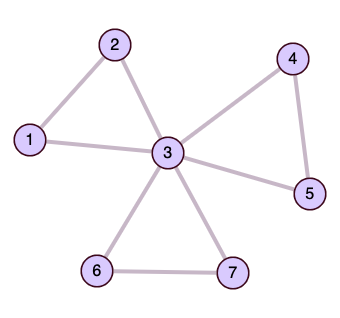
\includegraphics[width=0.3\textwidth]{flower_exp}
\end{center}

\textbf{Asymptotic magnitude from simulations:}
\\

$$\mathcal{M}_{3cycles-1vertex} = \frac{l \cdot t}{2} - 2$$


\textbf{Consistent with the 1st hypothesis:} when we glue 3 cycles with 1 vertex by inclusion-exclusion
principle: $$\mathcal{M}_{new \ graph} = \mathcal{M}_{cycle1} + \mathcal{M}_{cycle2} + \mathcal{M}_{cycle3}
- 2 \cdot \mathcal{M}_{connecting \ point} = \frac{l_1 \cdot t}{2} + \frac{l_2 \cdot t}{2} + \frac{l_3 \cdot t}{2} - 2
= \frac{l \cdot t}{2} - 2$$ 

\textbf{Consistent with the 2nd hypothesis:} see 4.3.3 section.

\subsubsection{Glued by 1 edge}

\begin{center}
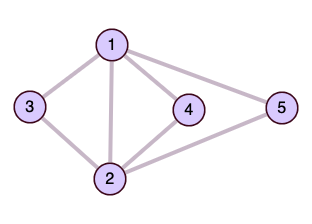
\includegraphics[width=0.3\textwidth]{3cicles_e_exp} \\ 
\end{center}

\textbf{Asymptotic magnitude from simulations:}
\\

$$\mathcal{M}_{3cycles-1edge} = \frac{l \cdot t}{2} - 2$$

\textbf{Simulations plot:}
\begin{center}
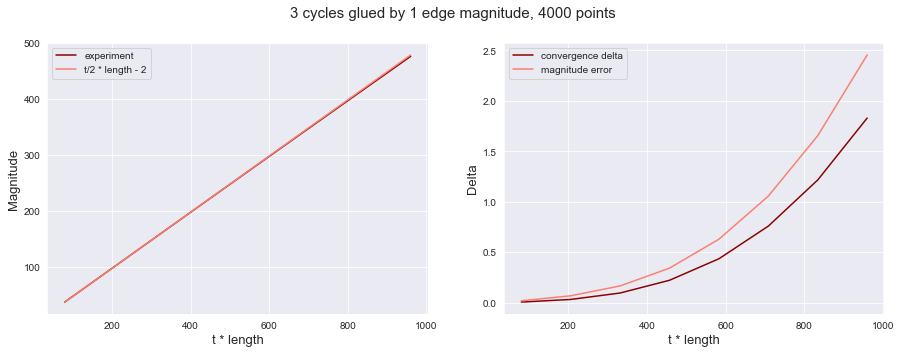
\includegraphics[width=\textwidth]{3cycles1edge_plot} \ \ \ \ \
\end{center}

\textbf{Consistent with the 1st hypothesis:} when we glue 3 cycles with 1 edge by inclusion-exclusion
principle: $$\mathcal{M}_{new \ graph} = \mathcal{M}_{cycle1} + \mathcal{M}_{cycle2} + \mathcal{M}_{cycle3}
- 2 \cdot \mathcal{M}_{connecting \ edge} = \frac{l_1 \cdot t}{2} + \frac{l_2 \cdot t}{2} + \frac{l_3 \cdot t}{2} - 2 \cdot (\frac{l_4 \cdot t}{2} + 1)
= \frac{l \cdot t}{2} - 2$$ 

\textbf{Consistent with the 2nd hypothesis:} $\chi = |\mathcal{V}| - |\mathcal{E}| = 5 - 7 = -2$.


\subsubsection{Glued by 2 edges}

\begin{center}
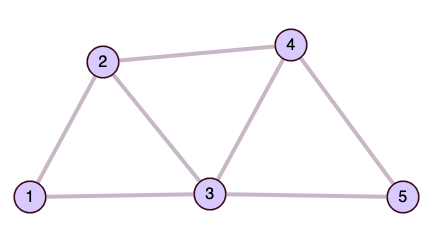
\includegraphics[width=0.4\textwidth]{3cicles_2e_exp} \ \ \ \ \
\end{center}

\textbf{Asymptotic magnitude from simulations:}
\\

$$\mathcal{M}_{3cycles-2edges} = \frac{l \cdot t}{2} - 2$$

\textbf{Simulations plot:}
\begin{center}
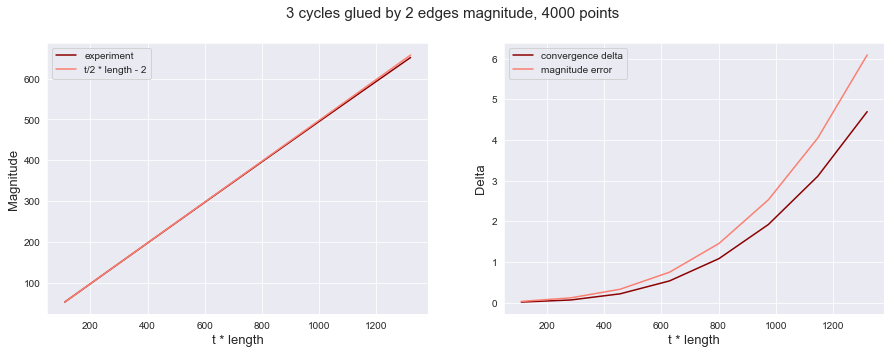
\includegraphics[width=\textwidth]{3cycles2edges_plot} \ \ \ \ \
\end{center}

\textbf{Consistent with the 1st hypothesis:} when we glue 3 cycles with 2 edges by inclusion-exclusion
principle: $$\mathcal{M}_{new \ graph} = \mathcal{M}_{cycle1} + \mathcal{M}_{cycle2} + \mathcal{M}_{cycle3}
- 2 \cdot \mathcal{M}_{connecting \ edges} = \frac{l_1 \cdot t}{2} + \frac{l_2 \cdot t}{2} + \frac{l_3 \cdot t}{2} - 2 \cdot (\frac{l_4 \cdot t}{2} + 1)
= \frac{l \cdot t}{2} - 2$$ 

\textbf{Consistent with the 2nd hypothesis:} $\chi = |\mathcal{V}| - |\mathcal{E}| = 5 - 7 = -2$.


\subsubsection{Glued by 3 edges}

\begin{center}
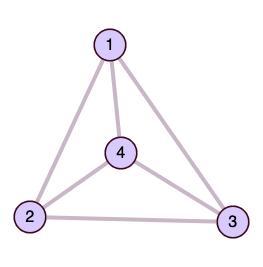
\includegraphics[width=0.3\textwidth]{3cicles_3e_exp}
\end{center}

\textbf{Asymptotic magnitude from simulations:}
\\

$$\mathcal{M}_{3cycles-3edges} = \frac{l \cdot t}{2} - 2$$

\textbf{Simulations plot:} 

\begin{center}
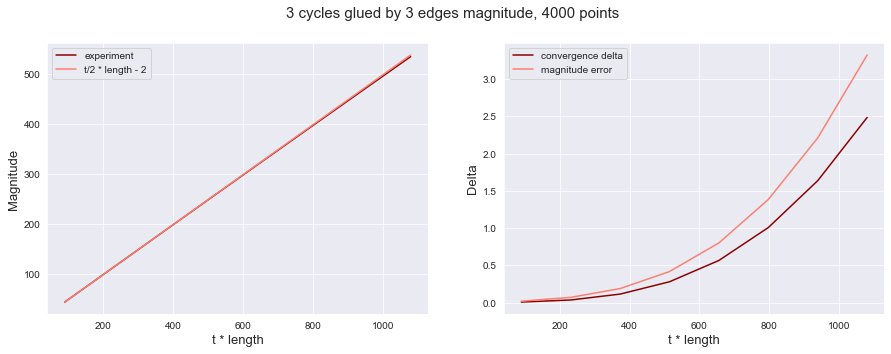
\includegraphics[width=\textwidth]{3cycles3edges_plot}
\end{center}

\textbf{Consistent with the 1st hypothesis:} when we glue 2 cycles with 1 vertex by inclusion-exclusion
principle: $$\mathcal{M}_{new \ graph} = \mathcal{M}_{cycle1} + \mathcal{M}_{cycle2} + \mathcal{M}_{cycle3}
- 3 \cdot \mathcal{M}_{connecting \ edges} + \mathcal{M}_{central \ point} =$$ 
$$ = \frac{l_1 \cdot t}{2} + \frac{l_2 \cdot t}{2} + \frac{l_3 \cdot t}{2} - 3 \cdot (\frac{l_4 \cdot t}{2} + 1) + 1 
= \frac{l \cdot t}{2} - 2$$ 

\textbf{Consistent with the 2nd hypothesis:} $\chi = |\mathcal{V}| - |\mathcal{E}| = 4 - 6 = -2$.

\subsection{Random graph}

\begin{center}
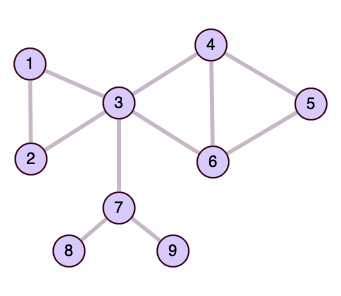
\includegraphics[width=0.4\textwidth]{random_exp}
\end{center}

\textbf{Asymptotic magnitude from simulations:}
\\

$$\mathcal{M}_{random} = \frac{l \cdot t}{2} - 2$$

\textbf{Simulations plot:} 

\begin{center}
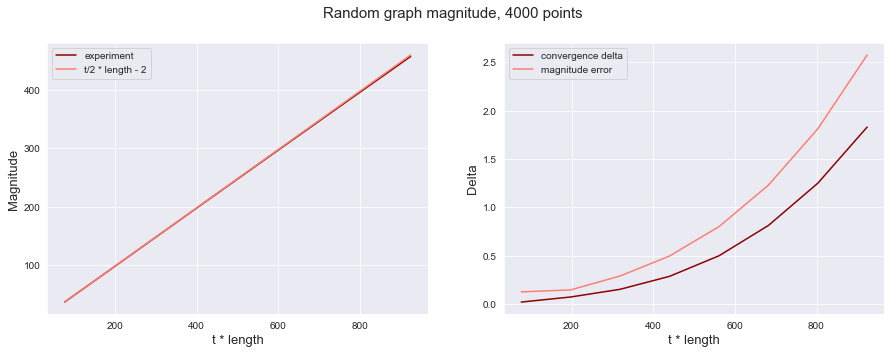
\includegraphics[width=\textwidth]{random_plot}
\end{center}

\textbf{Consistent with the 1st hypothesis} (easy to check by decomposing to cycles and trees). \\

\textbf{Consistent with the 2nd hypothesis:} $\chi = |\mathcal{V}| - |\mathcal{E}| = 9 - 11 = -2$, 

\section{Methods}

\subsection{Numeric computations}

Brief explanation of how we approximated magnitude functions (similar code can be found in \textcite{calc}):
first, we choose a few fixed $t = {t_1, t_2, ...}$; for each of them we approximate magnitude as 
$\lim \mathcal{M}_k(t)$ (see the pseudocode below). 

After that we plot connected ${(t_1, \mathcal{M}_k(t_1)), (t_2, \mathcal{M}_k(t_2)), ...}$
and try to guess the real $\mathcal{M}_{real}(t)$, to check the guess we plot
$|\mathcal{M}_{real}(t_i) - \mathcal{M}_k(t_i)|$ (right subplot). 

If it's close to 0 and behaves similar to the convergence delta, we conclude that we
asymptotically guessed the $\mathcal{M}_{real}$.  

All the results in this paper were obtained with the following numeric algorithm:\\

\begin{algorithm}
\caption{Magnitude function}\label{euclid}
\begin{algorithmic}[1]
    \Require $\mathcal{E}$ - list of edges of the graph \Comment{edge is represented as $(v_1, v_2, weight)$}
    \Procedure{Magnitude function}{$\mathcal{E}$}
    \State matrix D = bellman-ford-algorithm($\mathcal{E}$) \Comment{precompute pairwise shortest distances for all vertices} 
  \For{t $\in [10, 120]$}
    \For{number of points $\in [10, 4000]$}
      \State points = [points obtained from breaking edges to equal parts] \Comment lists length = number of points 
      \State matrix M: M[i][j] = $e^{-\text{t} \cdot \text{dist(points[i], points[j])}}$ \Comment dist uses D for vertices adjacent to points
      \State magnitude = sum(inverted(M))
      \State magnitude measures.append(magnitude)
    \EndFor
  \EndFor
    \State \textbf{return magnitude measures} \Comment used to plot magnitude(t) and check that it converges
\EndProcedure
\end{algorithmic}
\end{algorithm}

Range of t and number of points can be varied but note that scaling number of points
results in computation time (for [10, 4000] range it takes 10 min). Scaling t in
respect to graphs length (sum of weights) will result in worse convergence (since 
$e^{-t \cdot dist}$ becomes too small), in our experience to avoid that $t \cdot length$
should be $< 1000$. 

\begin{center}
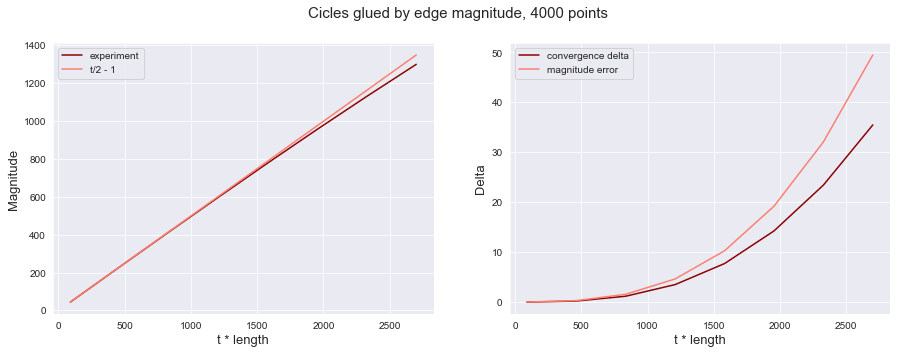
\includegraphics[width=1\textwidth]{too_high_t} \\ The plot above illustrates
    low precision of magnitude of too high $t \cdot length$.
    Note how errors go up to 40-50.
\end{center}

With $1 < t \cdot length < 1000$ and $10 < num points < 4000$ convergence rate is 
fast enough to expect real magnitude be in the neighbourhood:

\begin{center}
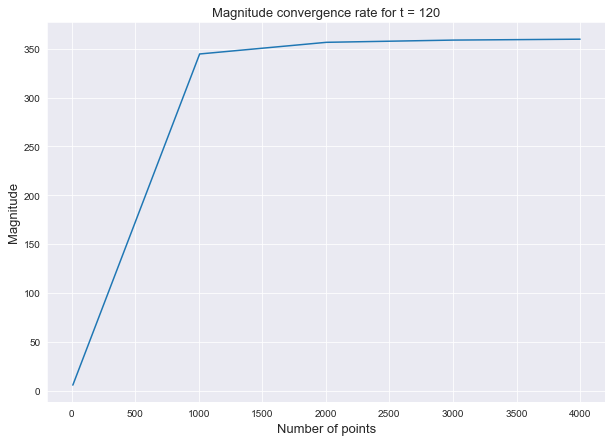
\includegraphics[width=0.6\textwidth]{convergence} \\ Illustration of the convergence
    rate, for an example graph. On the other plots in the work you can see that if 
    $t \cdot length < 1000$ convergence delta usually stays under $1-2$.
\end{center}



For different graph types we varied edges weights, so the plots in this report,
although each of them shows magnitude of one type of graph with fixed weights,
represents a set of graphs with the same configuration but different edges weights.
Varying weights in all the cases didn't influence magnitude function. 
\\ 

The code is implemented in Python with the use of Numpy for matrix computations,
for calculating inverted matrix we use numpy.linalg.inv. 
We tried using Scipy and other methods for matrix inversion: linsolve, methods
specified for positive definite or symmetric matrix. All those methods didn't give
any improvements nor with inversion precision, nor with the computational time. 
\\

Code can be found on \href{https://github.com/mmanchkin/magnitude}{Github} and in
\href{https://colab.research.google.com/drive/17Wlg996wKO1tZD9EBfn9G5qiL2nD_5LM?usp=sharing}{Colab},
we tried to make it user-friendly 
so to check any hypothesis it is enough to list all edges of the graph and call 2 methods
to calculate and plot comparison of guessed magnitude function and simulation result. 
\\

\subsection{Symbolic computations}

The other approach which we initially tried is symbolic computations.
Instead of measuring series of magnitudes for finite set of t and then guessing the real magnitude function,
we wanted to approximate it as \textbf{limit of function series over t}. 
\\

For a fixed metric graph we generated a sequence of it combinatorial subgraphs,
and then calculated magnitude directly as a function (not in small number of fixed t), using 
Sympy. \\

Unfortunately this approach didn't work out since this kind of computations are
way more complex than numerical ones and while symbolic computation for 3 points took around 4 sec,
for 4 points it worked for more than 10 min (note, how for numeric computations
we calculated magnitude for 4000 points). Also the results were not interpretable,
since number of terms in the magnitude failed to simplify and had a lot of terms 
(this is the expression for only 3 points):

\begin{center}
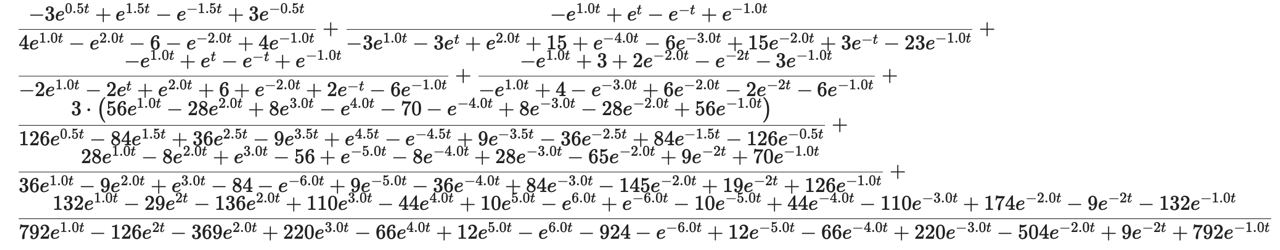
\includegraphics[width=0.8\textwidth]{many_terms}
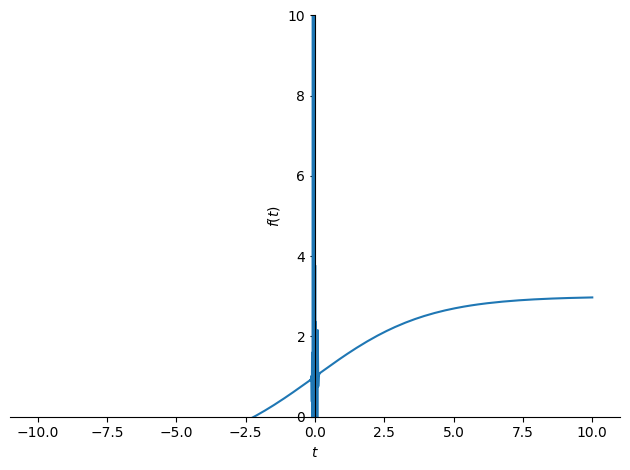
\includegraphics[width=0.5\textwidth]{func_plot} \\ Magnitude calculated as function in Sympy and its plot
\end{center}


\section{Conclusion}

We experimented with calculation of magnitude function of the metric graph and found 
some patterns in its behavior.
In this work we suggested two new hypothesis: 
\\

1. Magnitude function of the metric graph asymptotically satisfies inclusion-exclusion rule. \\

2. $\mathcal{M}_G(t) = \frac{t \cdot length}{2} + \chi(G) + q$, where $q \rightarrow 0$ and $\chi$ is Euler characteristic.
\\

The second hypothesis was proven for particular cases (e.g trees,
graphs with $\leq 1$ cycles, graphs glued by 1 vertex).
Both of the hypothesis were confirmed by all of the computer simulations. \\

Further work on the project might include searching for counterexample for one of 
the two hypothesis or finding generalized proof for any of them. \\

\printbibliography


% Проведем небольшой обзор возможностей \LaTeX. Далее идет обзорный кусок, который надо будет вырезать. Он приведен лишь для демонстрации возможностей \LaTeX.
%
% \section{Нумеруемый заголовок}
% Текст раздела
% \subsection{Нумеруемый подзаголовок}
% Текст подраздела
% \subsubsection{Нумеруемый подподзаголовок}
% Текст подподраздела
%
% \section*{Не нумеруемый заголовок}
% Текст раздела
% \subsection*{Не нумеруемый подзаголовок}
% Текст подраздела
% \subsubsection*{Не нумеруемый подподзаголовок}
% Текст подподраздела
%
%
% \paragraph{Заголовок абзаца} Текст абзаца
% Формулы в тексте набирают так $x = e^{\pi i}\sqrt{\text{формула}}$. Выключенные не нумерованные формулы набираются либо так:
% \[
% x = e^{\pi i}\sqrt{\text{формула}}
% \]
% Либо так
% $$
% x = e^{\pi i}\sqrt{\text{формула}}
% $$
% Первый способ предпочтительнее при подаче статей в журналы AMS, потому рекомендую привыкать к нему.
%
% Выключенные нумерованные формулы:
% \begin{equation}
% \label{Equation1}
% % \label{имя-метки} эта команда ставит метку, на которую потом можно сослаться с помощью \ref{имя-метки}. Метки можно ставить на все объекты, у которых есть автоматические счетчики (номера разделов, подразделов, теорем, лемм, формул и т.д.
% x = e^{\pi i}\sqrt{\text{формула}}
% \end{equation}
% Или не нумерованная версия
% \begin{equation*}
% x = e^{\pi i}\sqrt{\text{формула}}
% \end{equation*}
%
% Уравнение \ref{Equation1} радостно занумеровано.
%
% Лесенка для длинных формул
% \begin{multline}
% x = e^{\pi i}\sqrt{\text{очень очень очень длинная формула}}=\\
% \tr A - \sin(\text{еще одна очень очень длинная формула})=\\
% \cos z \Im \varphi(\text{и последняя длинная при длинная формула})
% \end{multline}
%
% Многострочная формула с центровкой
% \begin{gather}
% x = e^{\pi i}\sqrt{\text{очень очень очень длинная формула}}=\\
% \tr A - \sin(\text{еще одна очень очень длинная формула})=\\
% \cos z \Im \varphi(\text{и последняя длинная при длинная формула})
% \end{gather}
%
% Многострочная формула с ручным выравниванием. Выравнивание идет по знаку $\&$, который на печать не выводится.
% \begin{align}
% x = &e^{\pi i}\sqrt{\text{очень очень очень длинная формула}}=\\
% &\tr A - \sin(\text{еще одна очень очень длинная формула})=\\
% &\cos z \Im \varphi(\text{и последняя длинная при длинная формула})
% \end{align}
%
% \begin{theorem}
% Текст теоремы
% \end{theorem}
% \begin{proof}
% В специальном окружении оформляется доказательство.
% \end{proof}
%
% \begin{theorem}[Имя теоремы]
% Текст теоремы
% \end{theorem}
% \begin{proof}[Доказательство нашей теоремы]
% В специальном окружении оформляется доказательство.
% \end{proof}
%
% \begin{definition}
% Текст определения
% \end{definition}
%
% \begin{remark}
% Текст замечания
% \end{remark}
%
% \paragraph{Перечни:} Нумерованные
% \begin{enumerate}
% \item Первый
% \item Второй
% \begin{enumerate}
% \item Вложенный первый
% \item Вложенный второй
% \end{enumerate}
% \end{enumerate}
%
% Не нумерованные
%
% \begin{itemize}
% \item Первый
% \item Второй
% \begin{itemize}
% \item Вложенный первый
% \item Вложенный второй
% \end{itemize}
% \end{itemize}
\end{document}
